\documentclass[conference,10pt]{IEEEtran}
\usepackage{amsmath,amssymb,amsthm,bm}
\usepackage{graphicx}
\usepackage{booktabs}
\usepackage{algorithm}
\usepackage[noend]{algpseudocode}
\usepackage{tikz}
\usetikzlibrary{arrows.meta,positioning,fit,calc}
\usepackage{cite}
\usepackage{xcolor}
\usepackage[hidelinks]{hyperref}

\newtheorem{proposition}{Proposition}
\newtheorem{corollary}{Corollary}
\theoremstyle{remark}
\newtheorem{remark}{Remark}
\DeclareMathOperator{\diag}{diag}
\DeclareMathOperator{\vect}{vec}
\DeclareMathOperator{\sinc}{sinc}
\DeclareMathOperator{\tr}{tr}
\newcommand{\T}{\mathsf T}
\newcommand{\Hm}{\mathsf H}
\algrenewcommand\algorithmicrequire{\textbf{Input:}}
\algrenewcommand\algorithmicensure{\textbf{Output:}}

\begin{document}

\title{Timing-Only Channel Estimation and Equalization for OFDM Through a Dispersive Time-Modulated RIS}

\author{\IEEEauthorblockN{Yash Agrawal}
\IEEEauthorblockA{Birla Institute of Technology and Science, Pilani, India\\
p20240440@pilani.bits-pilani.ac.in}}

\maketitle

\begin{abstract}
A time-modulated reconfigurable intelligent surface (TM-RIS) switches its elements several times within each OFDM
symbol. The switching couples every received subcarrier to many transmitted ones, and with frequency-dispersive
elements the coupling matrix is neither diagonal nor Toeplitz. Existing TM-RIS designs treat this coupling as
interference, which caps the legitimate user's signal-to-interference ratio at $-4.8$\,dB for a 75\% duty cycle,
and the receiver for the dispersive model was left open. We show that grouping the harmonic expansion by element
state separates the coupling exactly into Toeplitz factors fixed by the switching timing, which the receiver knows,
and per-state input responses that absorb the propagation \emph{and} the element dispersion, which it does not.
From this separation we build, to our knowledge, the first pilot-based receiver for this channel: a low-rank
estimator that needs no element model, a blind estimator of the RIS clock offset that rests on the fact that an
offset is exactly an opposite delay of the two hops, and an exact matrix-free equalizer. In pre-registered tests
with 30 channels per point, the receiver comes within 0.1\,bit/s/Hz of perfect channel knowledge with two pilot
symbols on a shared-path channel and needs four to eight on 3GPP TDL-C. It beats every baseline we could build on
every channel and pilot count, including an ideal-element estimator with the same prior and basis-expansion
estimators with up to all harmonics and 32 pilot symbols. It decodes coded blocks within 0.14\,dB of perfect
knowledge, and it absorbs physical clock offsets with no significant rate loss.
\end{abstract}

\begin{IEEEkeywords}
Reconfigurable intelligent surface, time modulation, OFDM, intercarrier interference, channel estimation, equalization.
\end{IEEEkeywords}

\section{Introduction}
A time-modulated RIS (TM-RIS), or space-time-coding metasurface, switches each element several times within an OFDM
symbol~\cite{zhang2018}. The reflected signal then carries harmonics of the switching rate, which has been used for
waveform security and directional modulation~\cite{xu2023tmirs,tao2025gflownet}. For the user the surface serves,
the same harmonics move energy from transmitted subcarrier $m$ to received subcarrier $m+h$, so the channel matrix is
not diagonal. Iudice \emph{et al.}~\cite{iudice2026} recently derived a physically consistent model of this channel
with frequency-dispersive (finite-memory) elements, as real varactor cells are. They showed that the coupling survives
any cyclic prefix, that with dispersive elements the coupling matrix is not even Toeplitz. They assume the channel known
and name joint subcarrier equalization as future work~\cite[Sec.~V]{iudice2026}; channel estimation is not treated. Prior TM-RIS designs keep a one-tap receiver for the legitimate user and treat the coupling as
interference~\cite{xu2023tmirs,tao2025gflownet}. A blind eavesdropper attack~\cite{tao2025secure} relies on the
Toeplitz structure of ideal, frequency-flat switching, which dispersion breaks. Generic estimators of doubly selective
OFDM channels, such as the basis-expansion model (CE-BEM)~\cite{tang2007}, do not know where the coupling comes from:
they must estimate every harmonic. Because rectangular switching leaves a $1/h^2$ energy tail, they either truncate the
harmonics, which caps their accuracy, or keep all of them, which needs many pilots.

\emph{Novelty.} The receiver of a TM-RIS link knows \emph{how} the channel varies inside the symbol: the variation is
the switching pattern, which the network sets. It does not know the propagation or the exact element response. We turn
this observation into an exact structural statement and build the whole receiver on it. Our contributions are:
\begin{enumerate}
\item \emph{Timing--propagation separation} (Proposition~\ref{prop:sep}). Grouping the expansion of~\cite[eq.~(5)]{iudice2026}
by element state gives $\bm H=\sum_{q,s}\bm T_{q,s}\circ(\bm a^{\rm d}_q\bm v_{q,s}^{\T})$. The Toeplitz matrices
$\bm T_{q,s}$ depend only on the switching timing. The element dispersion enters only the per-state input response
$\bm v_{q,s}$, together with the unknown BS--RIS channel. The regrouping is elementary and we credit it to the anchor
model; what is new is what it implies for a receiver.
\item \emph{A receiver that needs no element model}: a low-rank, shared-subspace estimator of $\bm H$ that treats
$\bm v_{q,s}$ as unknown (Algorithm~\ref{alg:est}). Unlike~\cite{tao2025secure}, it does not rely on Toeplitz structure;
unlike CE-BEM, it never estimates harmonics separately.
\item \emph{Blind clock-offset recovery.} We prove that an offset between the RIS and the receiver is exactly an
opposite delay of the two hops (Proposition~\ref{prop:offset}), and we identify the offset physically
(Proposition~\ref{prop:phys}). This explains why a wrong offset overfits the pilots, and it leads to an estimator of the
offset and the delay reference by Bayesian evidence (Algorithm~\ref{alg:offset}).
\item \emph{A pre-registered evaluation}: pass/fail criteria fixed before each run, 30 channels per point, paired
confidence intervals, settings chosen on channels disjoint from the reported ones, the strongest baselines we could
build, and failures reported.
\end{enumerate}
We adopt and do not claim: the DPSS delay basis~\cite{slepian1978,zemen2005}, low-rank RIS channel
models~\cite{wang2020compressed}, matrix-free iterative equalization~\cite{hrycak2010} (exact here rather than a BEM
approximation), and evidence-based model selection~\cite{mackay1992}. The closest timing work, blind offset estimation
for RIS symbiotic radio~\cite{chen2024sr}, estimates the offset of a backscattered data stream from virtual subcarriers;
our receiver instead uses the known pattern and needs no idle subcarriers.

\emph{Notation:} $\circ$ and $\odot$ denote Hadamard products of matrices and vectors; $(\cdot)^{\T}$, $(\cdot)^{\Hm}$ and
$(\cdot)^{*}$ denote transpose, conjugate transpose and conjugate; $\sinc x=\sin(\pi x)/(\pi x)$; $\mathcal{CN}$ denotes the
circular complex Gaussian distribution.

\section{System Model}\label{sec:model}
\begin{figure}[t]\centering
\resizebox{\columnwidth}{!}{%
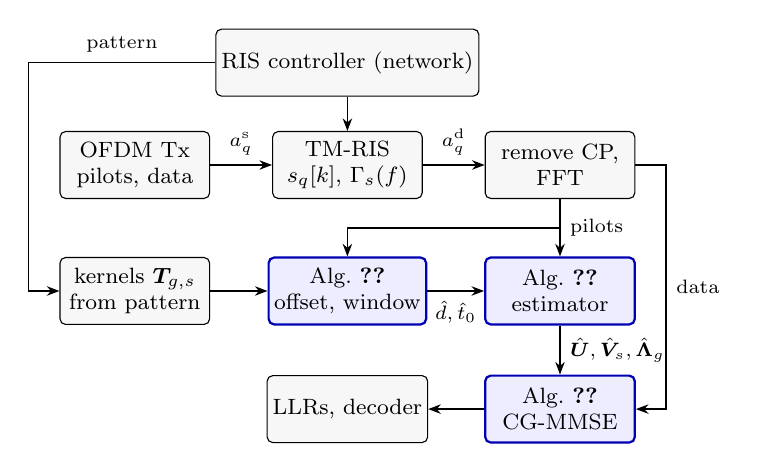
\begin{tikzpicture}[font=\footnotesize,
  box/.style={draw, rounded corners=2pt, align=center, minimum height=8.5mm, minimum width=19mm, inner sep=2pt, fill=gray!6},
  ours/.style={box, draw=blue!70!black, fill=blue!7, thick},
  ar/.style={-{Stealth[length=1.6mm]}, semithick}, lab/.style={font=\scriptsize}]
\node[box] (ctl) at (2.7,1.3) {RIS controller (network)};
\node[box] (tx) at (0,0) {OFDM Tx\\pilots, data};
\node[box] (ris) at (2.7,0) {TM-RIS\\$s_q[k]$, $\Gamma_s(f)$};
\node[box] (rx) at (5.4,0) {remove CP,\\FFT};
\node[box] (ker) at (0,-1.6) {kernels $\bm T_{g,s}$\\from pattern};
\node[ours] (off) at (2.7,-1.6) {Alg.~\ref{alg:offset}\\offset, window};
\node[ours] (est) at (5.4,-1.6) {Alg.~\ref{alg:est}\\estimator};
\node[ours] (eq) at (5.4,-3.1) {Alg.~\ref{alg:cg}\\CG-MMSE};
\node[box] (dec) at (2.7,-3.1) {LLRs, decoder};
\draw[ar] (tx) -- node[lab, above]{$a^{\rm s}_q$} (ris);
\draw[ar] (ris) -- node[lab, above]{$a^{\rm d}_q$} (rx);
\draw[ar] (ctl) -- (ris);
\draw[ar] (ctl.west) -- node[lab, above]{pattern} (-1.35,1.3) |- (ker.west);
\draw[ar] (rx) -- node[lab, right]{pilots} (est);
\draw[ar] ($(rx.south)!0.5!(est.north)$) -| (off.north);
\draw[ar] (ker) -- (off);
\draw[ar] (off) -- node[lab, below]{$\hat d,\hat t_0$} (est);
\draw[ar] (est) -- node[lab, right]{$\hat{\bm U},\hat{\bm V}_s,\hat{\bm\Lambda}_g$} (eq);
\draw[ar] (rx.east) -- (6.75,0) |- node[lab, right, pos=0.25]{data} (eq.east);
\draw[ar] (eq) -- (dec);
\end{tikzpicture}}
\caption{System and receiver. Highlighted blocks are the proposed algorithms. The receiver uses the switching pattern,
never the element model, and never forms the $M\times M$ coupling matrix.}\label{fig:sys}
\end{figure}

A base station (BS) transmits OFDM with $M$ subcarriers $f_m=f_c+m\Delta f$, $m\in\mathcal M=\{-M/2,\dots,M/2-1\}$,
useful duration $T_u=1/\Delta f$ and cyclic prefix (CP) $T_{\rm cp}$, to a user through a RIS of $Q$ elements
(Fig.~\ref{fig:sys}). Element $q$ follows a periodic pattern $s_q[k]\in\{1,2\}$, $k=0,\dots,K-1$, of period $T_u$: it is
in state $s_q[k]$ during slot $[kT_u/K,(k+1)T_u/K)$. The duty cycle $D$ is the fraction of slots in state 1. In state $s$
the element reflects with the single-resonance response of~\cite{iudice2026},
\begin{equation}
\Gamma_s(f)=-1+\frac{2\xi_{r,s}}{j2\pi(f-f_{0,s})+\xi_{r,s}+\xi_{i,s}},\label{eq:gamma}
\end{equation}
which for the published OpenRIS cell ($f_{0,1}=3.471$\,GHz, $f_{0,2}=3.710$\,GHz,
$\xi_{r,s}/2\pi=97.5$, $128.4$\,MHz, $\xi_{i,s}/2\pi=8.9$, $9.0$\,MHz~\cite[Tab.~I]{iudice2026}) drifts by about
$47^\circ$ in phase across a 100\,MHz carrier at $f_c=3.594$\,GHz (Fig.~\ref{fig:mech}a). It is far from the
frequency-flat $\pm1$ switch of earlier work. Let $a^{\rm s}_q(f)$ and $a^{\rm d}_q(f)$ be the BS--element and
element--user responses. When the CP covers the cascaded delay spread plus the element memory (13.8\,ns), the received
frequency-domain symbol is~\cite{iudice2026}
\begin{equation}
\bm y=\bm H\bm x+\bm w,\quad H_{\bar mm}=\sum_{q=1}^{Q}a^{\rm d}_q(f_{\bar m})\,b_q^{[\bar m-m]}(f_m)\,a^{\rm s}_q(f_m),\label{eq:io}
\end{equation}
where $\bm w\sim\mathcal{CN}(\bm 0,\sigma^2\bm I)$ and $b_q^{[h]}(f)$ is the $h$-th Fourier coefficient, over one period,
of the switched response of element $q$ at input frequency $f$. Equation~\eqref{eq:io} is the ground truth of our
evaluation. Its implementation agrees with an independent time-domain simulation (filter, gate, FFT, with no harmonic
algebra) to 0.27\% median relative error.

\emph{Assumptions.} Table~\ref{tab:assump} lists each assumption with its justification and where its violation is
evaluated. The receiver does \emph{not} assume~\eqref{eq:gamma}: it only defines the truth.

\begin{table}[t]\centering\footnotesize
\caption{Assumptions, justification, and where they are tested.}\label{tab:assump}
\begin{tabular}{@{}p{0.27\columnwidth}p{0.68\columnwidth}@{}}\toprule
Assumption & Justification; test of its violation\\\midrule
A1: pattern $s_q[k]$ known & The network drives the RIS controller, so the pattern is control information, like a pilot configuration. Without it the coupling cannot be told apart from propagation: a receiver that ignores one of two panels collapses to 1.15\,bit/s/Hz (Sec.~\ref{sec:res-hw}).\\
A2: generalized CP & Condition of~\cite{iudice2026}. Checked on the cascade: 3GPP TDL at 30 and 100\,ns is valid ($\le-56$\,dB of energy beyond the CP); 300\,ns is not and is out of scope.\\
A3: period $T_u$, aligned up to an offset $d$ & TM-IRS designs synchronize the pattern to the symbol~\cite{xu2023tmirs}; the residual offset is estimated (Sec.~\ref{sec:timing}).\\
A4: shared paths & A compact surface sees the same paths; this is what makes the factors low-rank. Tested with 3GPP TDL taps from random directions, spatially consistent CDL, 1024 elements and a near-field user.\\
A5: channel constant over a refresh block & The coherence time $0.423/f_D$~\cite{rappaport2002} spans 1188, 119 and 30 symbols at 3, 30 and 120\,km/h. Mobility is tested with the refresh interval selected under pilot overhead (Sec.~\ref{sec:res-mob}).\\
A6: $\sigma^2$ known; no mutual coupling & $\sigma^2$ is estimated from empty resource elements. Mutual coupling is ignored, as in~\cite{iudice2026}; this is a stated limitation.\\\bottomrule
\end{tabular}
\end{table}

\section{Structure of the Coupling}\label{sec:structure}
\begin{proposition}[Timing--propagation separation]\label{prop:sep}
For a $K$-slot pattern of period $T_u$, $b_q^{[h]}(f)=\sum_{s=1}^{2}t_{q,s}[h]\Gamma_s(f)$ with
\begin{equation}
t_{q,s}[h]=\frac{e^{-j\pi h/K}}{K}\sinc\Big(\frac hK\Big)\sum_{k:\,s_q[k]=s}e^{-j2\pi hk/K}.\label{eq:t}
\end{equation}
Hence, with $[\bm T_{q,s}]_{\bar mm}=t_{q,s}[\bar m-m]$ (Toeplitz), $\bm a^{\rm d}_q=[a^{\rm d}_q(f_m)]_m$ and
$\bm v_{q,s}=\bm\Gamma_s\odot\bm a^{\rm s}_q$,
\begin{equation}
\bm H=\sum_{q=1}^{Q}\sum_{s=1}^{2}\bm T_{q,s}\circ\big(\bm a^{\rm d}_q\bm v_{q,s}^{\T}\big).\label{eq:sep}
\end{equation}
\end{proposition}
\begin{proof}
In slot $k$ the element applies $\Gamma_{s_q[k]}(f)$, so its switched response is $\sum_s\Gamma_s(f)\mathbb 1_s(t)$, where
$\mathbb 1_s$ indicates the slots in state $s$. The $h$-th Fourier coefficient of the indicator of slot $k$ is
$\frac1{T_u}\int_{kT_u/K}^{(k+1)T_u/K}e^{-j2\pi ht/T_u}dt=\frac1Ke^{-j\pi h/K}\sinc(h/K)e^{-j2\pi hk/K}$. Summing over the
slots in state $s$ gives~\eqref{eq:t}. Substituting into~\eqref{eq:io}, $t_{q,s}$ depends on $\bar m-m$ only, which
gives~\eqref{eq:sep}.
\end{proof}

Proposition~\ref{prop:sep} has five consequences, which together define the receiver.

\begin{corollary}[No element model]\label{cor:nomodel}
The element response enters~\eqref{eq:sep} only through $\bm v_{q,s}$, which also contains the unknown BS--RIS
channel. Estimating $\bm v_{q,s}$ as an unknown absorbs the dispersion exactly; the receiver needs only the timing
kernels $\bm T_{q,s}$.
\end{corollary}

\begin{corollary}[One-tap ceiling]\label{cor:onetap}
For ideal $\pm1$ elements with a common pattern of duty $D$, $b^{[0]}=t_1[0]-t_2[0]=2D-1$, and Parseval's theorem gives
$\sum_h|b^{[h]}|^2=\frac1{T_u}\int_0^{T_u}|\pm1|^2dt=1$. A one-tap receiver collects the fraction $(2D-1)^2$ of the
reflected energy and sees the rest as interference, so its SIR is at most $(2D-1)^2/(1-(2D-1)^2)$: $-4.8$\,dB at $D=0.75$.
Joint equalization collects all of it.
\end{corollary}

\begin{corollary}[Harmonic tail]\label{cor:tail}
From~\eqref{eq:t}, $|t_{q,s}[h]|\le|\sinc(h/K)|$, which decays as $1/|h|$, so the energy outside $|h|\le H$ decays as
$1/H$. For $K=8$ and $D=0.75$ it is 3.4\%, 1.0\% and 0.32\% for $H=12$, 40 and 128 (Fig.~\ref{fig:mech}b). A model
truncated to $|h|\le12$ therefore has a normalized error floor of $10\log_{10}0.034=-14.7$\,dB, whatever its estimator.
\end{corollary}

\begin{corollary}[Fast products]\label{cor:fft}
$(\bm T\circ(\bm a\bm b^{\T}))\bm x=\bm a\odot(\bm T(\bm b\odot\bm x))$, and $\bm T\bm z$ is a linear convolution.
Hence $\bm H\bm x$ and $\bm H^{\Hm}\bm y$ cost $\mathcal O(QM\log M)$ with FFTs of length at least $3M-2$, and $\bm H$
is never formed.
\end{corollary}

\begin{proposition}[An offset is an opposite delay]\label{prop:offset}
If the switching runs $d$ slots late relative to the receiver's timing, each kernel becomes $\bm D\bm T\bm D^{*}$ with
$\bm D=\diag(e^{-j2\pi md/K})_{m\in\mathcal M}$, and
\begin{equation}
(\bm D\bm T\bm D^{*})\circ(\bm a\bm b^{\T})=\bm T\circ\big((\bm D\bm a)(\bm D^{*}\bm b)^{\T}\big).\label{eq:offset}
\end{equation}
Multiplying a frequency response by $\bm D$ delays it by $dT_u/K$; multiplying it by $\bm D^{*}$ advances it by the same amount.
\end{proposition}
\begin{proof}
A shift of $d$ slots multiplies the $h$-th coefficient by $e^{-j2\pi hd/K}=e^{-j2\pi\bar md/K}e^{j2\pi md/K}$ for
$h=\bar m-m$. This is~\eqref{eq:offset} entrywise.
\end{proof}

\begin{proposition}[Physical timing]\label{prop:phys}
Let the two hops have bulk delays $\tau_b$ and $\tau_u$, and let the receiver synchronize to the first cascaded arrival.
(i) If the RIS controller is locked to the signal arriving at the RIS, the synchronized $\bm H$ equals the one without
bulk delays. (ii) If it is locked to the BS clock, the synchronized $\bm H$ equals the one without bulk delays and with
offset $d=-\tau_b K/T_u$.
\end{proposition}
\begin{proof}
The delays multiply the input side by $e^{-j2\pi f_m\tau_b}$ and the output side by $e^{-j2\pi f_{\bar m}\tau_u}$;
synchronization multiplies the output by $e^{j2\pi f_{\bar m}(\tau_b+\tau_u)}$. In (i) the switching edges are delayed by
$\tau_b$, which by Proposition~\ref{prop:offset} contributes $e^{-j2\pi(\bar m-m)\Delta f\tau_b}$, and all phases cancel.
In (ii) the edges are not delayed, and what remains is the phase of an offset of $-\tau_b$.
\end{proof}
Both identities hold numerically to $7\cdot10^{-15}$. A practical RIS therefore sees either no offset or an offset
equal to its BS distance, tens to hundreds of nanoseconds; the latter costs 1.6/4.2\,bit/s/Hz at 20/30\,dB if
ignored (Table~\ref{tab:timing}).

\begin{figure}[t]\centering
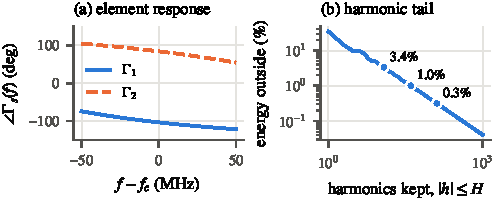
\includegraphics[width=\columnwidth]{fig_mechanism.pdf}
\caption{(a) Phase of the two states of the OpenRIS cell over the 100\,MHz carrier. (b) Fraction of the coupling energy
outside $|h|\le H$ for an ideal switch, $K=8$, $D=0.75$ (Corollary~\ref{cor:tail}).}\label{fig:mech}
\end{figure}

\section{The Receiver}\label{sec:receiver}
\subsection{Low-rank model with a delay prior}
Under A4, the user-hop response of element $q$ is $a^{\rm d}_q(f)=\sum_{\ell}g_\ell e^{-j\bm k\bm u_\ell^{\T}\bm r_q}
e^{-j2\pi f\tau_\ell}$, so $\bm a^{\rm d}_q=\bm E\bm\alpha_q$ with $\bm E=[e^{-j2\pi f_m\tau_\ell}]_{m,\ell}$ common to all
elements. Likewise $\bm v_{q,s}=\diag(\bm\Gamma_s)\bm E'\bm\beta_q$, where $\bm\beta_q$ (the input-hop path gains with the
element's geometric phases) is common to both states. Hence $[\bm a^{\rm d}_1,\dots,\bm a^{\rm d}_Q]$ has rank at most
the number of paths, whatever $Q$. Every hop response is delay-limited to a window $[t_0,t_0+\tau_{\max}]$, where
$\tau_{\max}$ also covers the element memory. We represent the responses with the first $L$ discrete prolate spheroidal
sequences (DPSS)~\cite{slepian1978,zemen2005}. These are the columns of $\bm F\in\mathbb C^{M\times L}$: the leading
eigenvectors of $R_{nm}=e^{-j\pi(n-m)\Delta f\tau_{\max}}\sinc((n-m)\Delta f\tau_{\max})$, the frequency correlation
of a response with delays uniform in the window. Their normalized eigenvalues $\bm\lambda$ serve as prior variances. Compressing the path gains to rank $r$ gives
$\bm a^{\rm d}_q=\bm F\bm U\tilde{\bm\alpha}_q$ and $\bm v_{q,s}=\bm F\bm V_s\tilde{\bm\beta}_q$. The second relation holds
because $\Gamma_s$ is smooth (memory 13.8\,ns): $\diag(\bm\Gamma_s)\bm E'$ stays delay-limited, so it lies in the same
DPSS span with a state-specific coefficient matrix $\bm V_s$, while $\tilde{\bm\beta}_q$ is shared by the two states. With
$G$ distinct patterns (groups $\mathcal G_g$) and rank $r$,~\eqref{eq:sep} becomes
\begin{equation}
\bm H=\sum_{g=1}^{G}\sum_{s=1}^{2}\bm T_{g,s}\circ\big((\bm F\bm U)\bm\Lambda_g(\bm F\bm V_s)^{\T}\big),\label{eq:model}
\end{equation}
with $\bm U,\bm V_s\in\mathbb C^{L\times r}$ and $\bm\Lambda_g=\sum_{q\in\mathcal G_g}\tilde{\bm\alpha}_q\tilde{\bm\beta}_q^{\T}
\in\mathbb C^{r\times r}$. The number of unknowns falls from up to $M^2$ to $3Lr+Gr^2$. An unswitched direct path is the
special case of equal input responses in both states (since $\bm T_{q,1}+\bm T_{q,2}=\bm I$), so~\eqref{eq:model}
contains it without change.

\subsection{Timing-only estimation (Algorithm~\ref{alg:est})}
Let pilot symbol $p$ be $\bm s_p$, with received $\bm y_p$, and let $\bm G_{g,s,p}=\bm T_{g,s}\diag(\bm s_p)\bm F$, computed
once by FFT. By Corollary~\ref{cor:fft},
\begin{equation}
\bm H\bm s_p=\sum_{g,s}\big[(\bm F\bm U\bm\Lambda_g)\circ(\bm G_{g,s,p}\bm V_s)\big]\bm 1_r,\label{eq:lin}
\end{equation}
which is linear in $\bm U$, in $[\bm V_1;\bm V_2]$ and in $\{\bm\Lambda_g\}$ when the other two are fixed. For each block
$\bm\theta$ the $N_p$ stacked pilots give $\bm y=\bm A_{\bm\theta}\bm\theta+\bm w$. With the prior
$\bm\theta\sim\mathcal{CN}(\bm 0,\bm P)$, $\bm P=\diag(\bm p)$, the columns of $\bm U$ and $\bm V_s$ carry variances
$\varsigma\bm\lambda$, with the scale $\varsigma$ set by moment matching on $\|\bm y\|^2$. The LMMSE update
\begin{equation}
\hat{\bm\theta}=\bm P^{1/2}\big(\bm P^{1/2}\bm A_{\bm\theta}^{\Hm}\bm A_{\bm\theta}\bm P^{1/2}+\sigma^2\bm I\big)^{-1}\bm P^{1/2}\bm A_{\bm\theta}^{\Hm}\bm y\label{eq:lmmse}
\end{equation}
stays well posed when some prior variances are tiny. Alternating~\eqref{eq:lmmse} over the blocks is non-convex, so the
initialization matters. Ignoring the coupling between groups gives a \emph{linear} model,
$\bm H\approx\sum_s\bar{\bm T}_s\circ(\bm F\bm C_s\bm F^{\T})$ with $\bar{\bm T}_s=\sum_g\bm T_{g,s}$, which is exact for
$G=1$. Its LMMSE estimate with prior $\varsigma(\bm\lambda\otimes\bm\lambda)$, followed by a rank-$r$ SVD
$[\hat{\bm C}_1\;\hat{\bm C}_2]\approx\bm Y\bm\Sigma\bm W^{\Hm}$, initializes the factors. From this initialization ALS
converges in one or two iterations; random initializations end 3--5 times worse.

\begin{algorithm}[t]\caption{Timing-only low-rank estimation}\label{alg:est}
\begin{algorithmic}[1]
\Require pilots $\{\bm y_p,\bm s_p\}$; kernels $\bm T_{g,s}$; $\bm F,\bm\lambda$; $\sigma^2$; rank $r$; iterations $I$
\State $\bm G_{g,s,p}\gets\bm T_{g,s}\diag(\bm s_p)\bm F$ by FFT
\State $[\hat{\bm C}_1,\hat{\bm C}_2]\gets$ LMMSE of the linear model; rank-$r$ SVD $\to\bm U=\bm Y_r\bm\Sigma_r^{1/2}$, $[\bm V_1;\bm V_2]=\bm W^{*}_r\bm\Sigma_r^{1/2}$, $\bm\Lambda_g=\bm I$
\For{$i=1,\dots,I$}
\State $\{\bm\Lambda_g\}\gets$ ridge least squares on~\eqref{eq:lin}; $\bm U\gets$~\eqref{eq:lmmse}; $[\bm V_1;\bm V_2]\gets$~\eqref{eq:lmmse}
\EndFor
\Ensure factors of~\eqref{eq:model} ($\bm H$ is not formed)
\end{algorithmic}
\end{algorithm}

\emph{Why two pilot symbols can suffice.} At $M=256$ with $L=16$ and $r=8$ there are 448 unknowns against 512
observations from two pilot symbols, yet the problem is well determined because the prior concentrates each hop on
about $M\Delta f\tau_{\max}+1$ dimensions. We measured the effective degrees of freedom of the linear stage, the trace of
its LMMSE hat matrix: 19--27 at 20\,dB and 23--33 at 30\,dB for 1--8 pilot symbols, against 256--2048 observations. With
two pilot symbols the achieved coupling-matrix error is 5--6\,dB above the Bayesian bound under the assumed prior
($-26.4$ vs $-32.4$\,dB at 20\,dB). The gap is not estimator suboptimality: real channels do not follow the
uniform-delay prior. An earlier version kept the linear estimate whenever it fitted the pilots better. On fresh 3GPP
channels this rule was an overfitting trap (chosen in 37--57\% of channels at 30\,dB, worse rate), so
Algorithm~\ref{alg:est} always returns the low-rank estimate.

\subsection{Blind clock offset and delay reference (Algorithm~\ref{alg:offset})}\label{sec:timing}
By Proposition~\ref{prop:offset} a candidate offset $d$ replaces each kernel by $\bm D_d\bm T_{g,s}\bm D_d^{*}$, and a
window start $t_0$ replaces $\bm F$ by $\bm F_{t_0}=\diag(e^{-j2\pi m\Delta ft_0})\bm F$. For each candidate the linear stage
is a Gaussian model, $\bm y=\bm\Phi\bm c+\bm w$ with $\bm c\sim\mathcal{CN}(\bm 0,\bm P)$, and its log-evidence is, up
to a constant,
\begin{equation}
\mathcal E(d,t_0)=-\bm y^{\Hm}\bm C^{-1}\bm y-\log\det\bm C,\qquad \bm C=\bm\Phi\bm P\bm\Phi^{\Hm}+\sigma^2\bm I.\label{eq:ev}
\end{equation}
With the Cholesky factor $\bm R^{\Hm}\bm R=\sigma^{-2}\bm P^{1/2}\bm\Phi^{\Hm}\bm\Phi\bm P^{1/2}+\bm I$ and the Woodbury
identity, $\log\det\bm C=MN_p\log\sigma^2+2\sum_i\log R_{ii}$ and
$\bm y^{\Hm}\bm C^{-1}\bm y=\sigma^{-2}\|\bm y\|^2-\sigma^{-4}\|\bm R^{-\Hm}\bm P^{1/2}\bm\Phi^{\Hm}\bm y\|^2$, so the
evidence costs one $2L^2$-dimensional factorization per candidate.

\emph{Why the evidence.} By~\eqref{eq:offset}, a wrong offset can still explain the pilots, through a delayed user hop
and an advanced BS hop. The pilot residual is therefore nearly flat in $d$ for physical offsets below about 100\,ns.
For such offsets, the residual of the advanced response after projection onto the delay basis is only $2.7\cdot10^{-4}$
at 100\,ns (relative). A wrong offset thus \emph{overfits}: it fits through improbable shifted responses. The log-determinant
in~\eqref{eq:ev} penalizes exactly this. With two held-out pilot symbols, the offset that minimizes the held-out
residual agrees with the evidence maximizer within 0.005 slot in 93\% of channels. The window start must be estimated
too. After synchronization the first arrivals of the two hops sum to zero up to the offset, so a window that starts after
the true reference cannot hold both hops; a synchronization error has the same effect. The evidence of different priors
is directly comparable, so $t_0$ is chosen jointly with $d$.

\begin{algorithm}[t]\caption{Offset and delay reference by evidence}\label{alg:offset}
\begin{algorithmic}[1]
\Require pilots; nominal kernels; $\bm F,\bm\lambda$; $\sigma^2$; $\mathcal T_0=\{-150,-75,0,75\}$\,ns
\For{$t_0\in\mathcal T_0$}
\State $d_0\gets\arg\max_d\mathcal E(d,t_0)$ on a 41-point grid over $[-\frac12,\frac12]$ slot
\State $\hat d_{t_0}\gets$ golden-section search of $\mathcal E(\cdot,t_0)$ on $d_0\pm0.025$ (14 steps)
\EndFor
\Ensure $(\hat d,\hat t_0)=\arg\max_{t_0}\mathcal E(\hat d_{t_0},t_0)$; run Algorithm~\ref{alg:est} with them
\end{algorithmic}
\end{algorithm}

\subsection{Matrix-free equalization and complexity}
The MMSE symbol estimate solves $(\hat{\bm H}^{\Hm}\hat{\bm H}+\sigma^2\bm I)\bm x=\hat{\bm H}^{\Hm}\bm y$. We solve it by
conjugate gradients (CG), as in~\cite{hrycak2010}. Each product goes through~\eqref{eq:model}: for $G=1$, the FFTs of all
$r$ columns and all data symbols form one batched call per state, the two states are summed in the frequency domain,
and one batched inverse FFT follows (Algorithm~\ref{alg:cg}). Unlike the BEM approximation in~\cite{hrycak2010}, this
representation is exact. The stopping tolerance was chosen by a pre-registered sweep. With $\epsilon=10^{-2}$ the
symbol error rate (SER) is 1.15 times the dense solve's at $M=3276$; with $\epsilon=3\cdot10^{-3}$ it is within 2\% of it at
every $M$ from 1024 to 6552, after 8--20 iterations.

\begin{algorithm}[t]\caption{Matrix-free CG-MMSE equalization}\label{alg:cg}
\begin{algorithmic}[1]
\Require data $\bm Y_d$ (symbols as columns); factors of $\hat{\bm H}$; $\sigma^2$; $\epsilon=3\cdot10^{-3}$; $i_{\max}=50$
\State $\bm B\gets\hat{\bm H}^{\Hm}\bm Y_d$; $\bm X\gets\bm 0$; $\bm R\gets\bm B$; $\bm P\gets\bm R$
\For{$i=1,\dots,i_{\max}$} \Comment{per column}
\State $\bm Q\gets\hat{\bm H}^{\Hm}(\hat{\bm H}\bm P)+\sigma^2\bm P$ \Comment{batched FFT products}
\State $\alpha\gets\|\bm r\|^2/\bm p^{\Hm}\bm q$; $\bm x\gets\bm x+\alpha\bm p$; $\bm r'\gets\bm r-\alpha\bm q$
\State \textbf{if} $\|\bm r'\|/\|\bm b\|<\epsilon$ for all columns \textbf{break}
\State $\bm p\gets\bm r'+(\|\bm r'\|^2/\|\bm r\|^2)\bm p$; $\bm r\gets\bm r'$
\EndFor
\end{algorithmic}
\end{algorithm}

\emph{Complexity} (complex multiply--adds). One ALS iteration costs
$\sum_{n\in\{Lr,2Lr,Gr^2\}}(MN_pn^2+n^3/3)$; the linear stage costs $MN_p(2L^2)^2+(2L^2)^3/3$. For $G=1$, $r=8$, $N_p=2$
and 20 iterations this totals $5.7\cdot10^8$ at $M=256$ and $3.9\cdot10^{10}$ at the full $M=3276$. One CG iteration
costs two products of $\mathcal O(rM\log M)$, together about $1.7\cdot10^7$ operations at $M=3276$, so a symbol costs at most
$3.4\cdot10^8$ with 20 iterations. The dense alternative forms $\hat{\bm H}$ (172\,MB at $M=3276$, 687\,MB at $M=6552$) and
factors $\hat{\bm H}^{\Hm}\hat{\bm H}+\sigma^2\bm I$ once per estimate ($4.7\cdot10^{10}$ operations), after which each symbol
costs $\mathcal O(M^2)$. By operation count CG would be cheaper for blocks of up to about 140 symbols per estimate.
Measured wall-clock time is less favourable, because the dense factorization runs as optimized level-3 BLAS while CG
is memory-bound. On an otherwise idle 4-thread CPU (MATLAB R2026a, $\epsilon=3\cdot10^{-3}$, $M=3276$, 20\,dB), dense
equalization of $N=1$, 12, 40 and 120 symbols per estimate took 2.51, 2.54, 2.58 and 2.78\,s including the factorization,
and CG took 0.23, 2.51, 8.2 and 23.8\,s; the symbol error rate of CG was within 2\% of dense. The measured break-even is
therefore about 12 symbols per estimate (6 at $M=2048$). That is the refresh interval selected at 30 and 120\,km/h
(Sec.~\ref{sec:res-mob}), where CG is the faster choice. For slow channels with 40--120 symbols per estimate, dense
equalization is 3--9$\times$ faster when its memory is available. CG's lasting advantage is memory linear in $M$: at
$M=6552$ it equalized 120 symbols in 51\,s without forming the 687\,MB matrix.
Warm-starting a refresh from
the previous factors (two ALS iterations, no linear stage) took 1.4\,s against 12.5\,s from scratch, with the same SER.

\section{Evaluation}\label{sec:eval}
\emph{Setup.} We use the n78 carrier with $\Delta f=30$\,kHz, $T_{\rm cp}=2.34\,\mu$s, $Q=16$ elements ($4\times4$,
$\lambda/2$), $K=8$, $D=0.75$, identical patterns unless stated, and the OpenRIS cell~\eqref{eq:gamma}. Comparisons use
$M=256$ (central 128 subcarriers scored); full-band results use $M=3276$. Channels:
\begin{itemize}
\item a \emph{shared-path} channel: per hop, one line-of-sight and five scattered paths, 30\,ns rms, Rician factor 10\,dB;
\item 3GPP TDL-A/C/D~\cite{tr38901} at 100\,ns, with taps from random directions.
\end{itemize}
Pilots are QPSK pilot symbols. The estimator uses $\tau_{\max}=0.3\,\mu$s, $L=16$, $r=8$ on the shared-path channel and
$\tau_{\max}=1\,\mu$s, $L=\lceil M\Delta f\tau_{\max}\rceil+10$, $r=16$ on TDL. These hyperparameters were frozen before
the tests below. The metric is the achievable rate of the MMSE filter $\bm W$ built from the estimate and applied to the
\emph{true} channel: with $\bm G=\bm W\bm H$, $\mathrm{SINR}_m=|G_{mm}|^2/(\sum_{n\ne m}|G_{mn}|^2+\sigma^2\|\bm w_m\|^2)$,
and $R=\mathrm{mean}_m\log_2(1+\mathrm{SINR}_m)$. The \emph{loss} is $R$ with perfect channel state information (CSI)
minus $R$ with the estimate. Each test was pre-registered with its pass criterion and uses 30 independent channels per
point; intervals are paired 95\% $t$-intervals.

\emph{Baselines.} All baselines get the same pilots, the same prior family and, for fairness, three equalizers each:
naive MMSE, robust MMSE with the estimation-error power taken from the pilot residual, and robust MMSE with the
oracle error power. Figures show the residual-based robust MMSE, which is usable in practice; paired comparisons
take, per channel, the best over all baselines and all three equalizers.
\begin{itemize}
\item \emph{One-tap}: today's OFDM receiver.
\item \emph{Ideal-element LMMSE}: the strongest estimator that assumes the textbook element, $\bm H=(\bm T_1-\bm T_2)\circ
(\bm F\bm C\bm F^{\T})$ with our prior.
\item \emph{CE-BEM}~\cite{tang2007}: $\bm H=\sum_{|h|\le H_b}\bm S_h\diag(\bm F_2\bm c_h)$ with up to all $2M-1$
harmonics, solved matrix-free (equal to the dense solver to $7\cdot10^{-9}$); with all harmonics it is run from eight
pilot symbols.
\item \emph{OMP}~\cite{tropp2007} over a harmonic$\times$delay dictionary.
\end{itemize}

\subsection{Comparison with the strongest baselines}\label{sec:res-fair}
\begin{figure*}[t]\centering
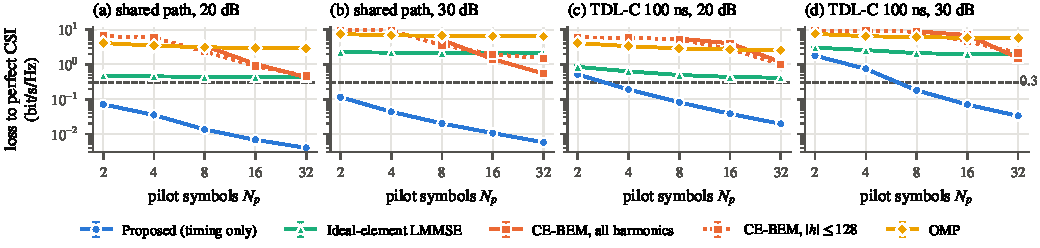
\includegraphics[width=\textwidth]{fig_fair.pdf}
\caption{Loss to perfect CSI versus pilot symbols (30 channels, 95\% intervals, residual-based robust MMSE for every
estimator). Dashed line: 0.3\,bit/s/Hz. Perfect-CSI rates: 6.62/9.92 (shared path), 6.20/9.38\,bit/s/Hz (TDL-C) at 20/30\,dB.}\label{fig:fair}
\end{figure*}
Fig.~\ref{fig:fair} gives the loss to perfect CSI. The proposed estimator is the only one that comes within 0.3\,bit/s/Hz
with at most 32 pilot symbols. It needs two on the shared-path channel (loss $0.07\pm0.02$ / $0.11\pm0.03$ at 20/30\,dB)
and four on TDL-C ($0.19$ at 20\,dB; eight for $0.18$ at 30\,dB); the longer delay window of TDL means more unknowns. The
one-tap receiver is capped by Corollary~\ref{cor:onetap} (0.43\,bit/s/Hz at both SNRs).

The strongest baseline is the ideal-element LMMSE. With eight or more pilot symbols it loses 0.4--0.5\,bit/s/Hz at
20\,dB but 1.9--2.2 at 30\,dB, and more pilots do not help it. This is the signature of a \emph{model} error: at high SNR the dispersion it ignores dominates.
It is the quantitative case for Corollary~\ref{cor:nomodel}. CE-BEM stalls when truncated (Corollary~\ref{cor:tail}). With all
harmonics it has 8687 unknowns at $M=256$, and even with 32 pilot symbols it reaches only the ideal-element level (0.43 at 20\,dB on the shared-path channel, 1.17 on TDL-C). Our receiver with two pilot symbols is
therefore better than full CE-BEM with 32. Paired per channel against the best baseline on that channel (minimum over
all baselines and equalizers), ours gains $0.41\pm0.02$ / $2.16\pm0.04$\,bit/s/Hz at $N_p=2$ on the shared-path channel
and $0.30\pm0.06$ / $1.14\pm0.25$ on TDL-C. At every pilot count from 2 to 32 the gain is 0.3--0.4 at 20\,dB and
0.5--2.2 at 30\,dB, and every interval excludes zero. If the detector does not know $G_{mm}$ and uses its estimate,
every loss grows by at most 0.15. One pre-registered sanity check failed. Truncated CE-BEM still loses rate from 20 to
30\,dB even with the oracle robust equalizer, because a scalar error power cannot describe an error concentrated on
the missing harmonics.

\subsection{No element model: robustness beyond the generating model}\label{sec:res-model}
A receiver tested on data from its own model can look better than it is. Table~\ref{tab:robust} runs the estimator
\emph{unchanged} on data that violate its structure, paired with the same channel without the change. In every case the
extra loss stays within 0.05\,bit/s/Hz, which passes the pre-registered bar of 0.3. Element-to-element resonance spread
of 5--20\,MHz costs 0.06--0.15\,bit/s/Hz. A six-parameter fit of the element model is not better than timing-only
($+0.08\pm0.05$ worse at 30\,dB) and fails with element spread ($+0.73\pm0.43$). On a 16-element surface the linear first
stage provides most of the gain (loss 0.10/0.23 at $N_p=2$); the low-rank step and one decision-directed pass reduce it
to 0.07/0.11 and 0.02/0.03. The low-rank property itself matters most for large surfaces: the effective rank of the
true element-domain matrix (99\% energy, CDL-C, 98\,MHz, beam squint) is 5, 9, 13 and 16 for $Q=16$, 64, 256 and 1024.

\begin{table}[t]\centering\footnotesize
\caption{Estimator unchanged on data violating its model: relative change of $\bm H$ and extra loss (bit/s/Hz, paired, 30 channels).}\label{tab:robust}
\setlength{\tabcolsep}{3pt}
\begin{tabular}{@{}lccc@{}}\toprule
Violation & $\Delta\bm H$ & 20\,dB & 30\,dB\\\midrule
Time-domain truth & 0.006 & $-0.004\pm0.005$ & $+0.006\pm0.009$\\
Switching transients & 0.001 & $+0.001\pm0.001$ & $+0.003\pm0.006$\\
State-dep.\ output, $\epsilon=0.2$ & 0.40 & $\le0.004$ & $+0.034$\\
Joint-state coupl., $\kappa=0.08$ & 0.29 & $\le0.002$ & $+0.015$\\
Resonance spread 10\,MHz & 0.18 & $+0.003\pm0.008$ & $+0.046\pm0.044$\\
Beam squint, $Q=256$ & 0.016 & $\le0.001$ & $-0.002$\\\bottomrule
\end{tabular}
\end{table}

\subsection{Timing}\label{sec:res-timing}
Table~\ref{tab:timing} tests Algorithm~\ref{alg:offset} with physical bulk delays ($\tau_b\sim\mathcal U(50,300)$\,ns,
$\tau_u\sim\mathcal U(30,300)$\,ns). A BS-clock-locked RIS needs the search, and with the search the rate is within
noise of known timing. An incident-signal-locked RIS needs no search, and running it anyway costs nothing significant.
A synchronization error of up to $\pm150$\,ns breaks a fixed delay window, but not the jointly chosen one. Is the evidence
necessary? On a fine grid the pilot residual of the full low-rank estimate also finds the offset with two or more pilot
symbols (not significantly worse). With a single pilot symbol it overfits: it is worse by $1.49\pm0.56$ / $2.83\pm1.19$\,bit/s/Hz,
while the evidence stays within $0.03$ of known timing at 20\,dB. The evidence is also 5--58 times cheaper per search
(3.2 vs 17.2\,s at $M=256$; 11.7 vs 674\,s on TDL-C), because it needs no low-rank estimate per candidate. Random
per-edge jitter cannot be estimated. It must stay below about 4\,ns rms at 30\,dB (20\,ns at 20\,dB), whereas ordinary
clocks have picosecond jitter.

\begin{table}[t]\centering\footnotesize
\caption{Timing: losses and paired differences (bit/s/Hz, 30 channels).}\label{tab:timing}
\setlength{\tabcolsep}{3pt}
\begin{tabular}{@{}lcc@{}}\toprule
 & 20\,dB & 30\,dB\\\midrule
BS-clock RIS, offset ignored & 1.62 & 4.23\\
\quad Alg.~\ref{alg:offset} minus known offset & $+0.011\pm0.019$ & $+0.033\pm0.066$\\
Incident-locked: Alg.~\ref{alg:offset} minus none & $+0.001\pm0.007$ & $+0.040\pm0.082$\\
Sync error $\le150$\,ns, fixed window & 0.22 & 1.16\\
\quad window chosen by evidence & $0.05\pm0.05$ & $0.05\pm0.08$\\
$N_p=1$: residual minus evidence & $1.49\pm0.56$ & $2.83\pm1.19$\\\bottomrule
\end{tabular}
\end{table}

\subsection{Full band and coded link}
At the full band ($M=3276$, 30 channels) the SER with two pilot symbols is 1.10 [1.06, 1.15] times the perfect-CSI SER
at 20\,dB with 16-QAM and 1.37 [1.18, 1.86] times at 28\,dB with 64-QAM (95\% clustered-bootstrap intervals). One
decision-directed pass brings these to 1.05 and 1.12. CE-BEM ($|h|\le8$) is 18 and 32 times worse; the one-tap
receiver's SER is 0.84 and 0.96. Fig.~\ref{fig:bler} shows the coded link: a rate-1/2 convolutional code, 16-QAM,
max-log LLRs from each receiver's own estimate, and 2000 blocks per point. The proposed receiver crosses 10\% block
error rate (BLER) at 8.51\,dB against 8.37\,dB with perfect CSI, a gap of $0.14$\,dB [0.09, 0.20]. One-tap never
decodes, and truncated CE-BEM floors at 34\%.

\begin{figure}[t]\centering
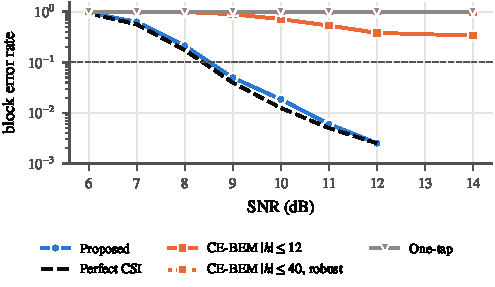
\includegraphics[width=\columnwidth]{fig_bler.pdf}
\caption{Coded BLER, $N_p=2$, 2000 blocks per point. Gap to perfect CSI at 10\% BLER: 0.14\,dB [0.09, 0.20].}\label{fig:bler}
\end{figure}

\subsection{Mobility and pilot overhead}\label{sec:res-mob}
When the user moves, only the RIS--user hop changes. Each path rotates by $e^{j2\pi\nu_\ell nT_s}$ between symbols and
also mixes subcarriers within a symbol. That mixing is $-60$, $-47$ and $-34$\,dB below the signal at 3, 30 and
120\,km/h, so the main effect is the ageing of the estimate. With $N_p$ pilot symbols every $N$ symbols, the net rate is
$R_{\rm net}=\frac{1}{N}\sum_{n=N_p}^{N-1}R(n)$, where $R(n)$ uses the estimate on symbol $n$ with one common phase
corrected per symbol, as 5G phase-tracking pilots do. Table~\ref{tab:overhead} selects $(N_p,N)$ and, for CE-BEM,
the harmonic range on 20 channels, and reports them on 20 \emph{other} channels. Ours beats the best CE-BEM in all 24
cases, by 1.0--3.9\,bit/s/Hz, with every interval above zero; CE-BEM needs 16--32 pilot symbols and so pays far more
overhead. Selecting on the reported channels instead changes the numbers by at most 0.13. After paying for its
pilots, ours keeps 75--93\% of the perfect-CSI rate on the shared path and 73--88\% on TDL at 3\,km/h. On TDL at
120\,km/h it keeps only 46--66\%: the coherence time is 30 symbols, so the selected design refreshes every 6 symbols
with one pilot symbol, and the overhead and the ageing estimate both cost rate. Slow channels prefer two (shared path)
or four (TDL) pilot symbols every 40--120 symbols; at 30 and 120\,km/h one or two pilot symbols every 6--30 symbols.
High mobility is therefore a limit of this pilot-based design, not of the coupling model. Two decision-directed trackers
(LMMSE and Kalman) were worse than reusing the pilot estimate, because wrong decisions accumulate after about ten
symbols.

\begin{table}[t]\centering\footnotesize
\caption{Net throughput after pilot overhead (bit/s/Hz), $(N_p,N)$ selected on 20 channels and reported on 20 disjoint channels; ours $-$ CE-BEM paired, 95\% interval.}\label{tab:overhead}
\setlength{\tabcolsep}{2.2pt}
\begin{tabular}{@{}lccccccc@{}}\toprule
 & & \multicolumn{3}{c}{20\,dB} & \multicolumn{3}{c}{30\,dB}\\
Channel & km/h & ours & BEM & diff. & ours & BEM & diff.\\\midrule
%ROWS-BEGIN (generated by figures/analyse_heldout.py)
Shared & 3 & 6.24 & 5.24 & $1.01\pm0.14$ & 8.99 & 7.34 & $1.65\pm0.34$\\
Shared & 30 & 5.97 & 4.40 & $1.57\pm0.30$ & 8.56 & 5.42 & $3.14\pm0.40$\\
Shared & 120 & 5.26 & 3.15 & $2.11\pm0.30$ & 7.30 & 3.38 & $3.92\pm0.53$\\
\midrule
TDL-A & 3 & 5.38 & 3.71 & $1.67\pm0.17$ & 7.37 & 4.88 & $2.49\pm0.21$\\
TDL-A & 30 & 4.56 & 1.60 & $2.97\pm0.13$ & 5.51 & 1.68 & $3.84\pm0.27$\\
TDL-A & 120 & 3.81 & 1.08 & $2.73\pm0.28$ & 4.35 & 1.07 & $3.27\pm0.58$\\
\midrule
TDL-C & 3 & 5.34 & 3.61 & $1.74\pm0.16$ & 7.23 & 4.81 & $2.41\pm0.27$\\
TDL-C & 30 & 4.53 & 1.65 & $2.88\pm0.29$ & 5.53 & 1.81 & $3.72\pm0.42$\\
TDL-C & 120 & 3.88 & 0.75 & $3.13\pm0.31$ & 4.61 & 0.74 & $3.88\pm0.54$\\
\midrule
TDL-D & 3 & 5.17 & 3.61 & $1.56\pm0.17$ & 6.80 & 4.75 & $2.05\pm0.41$\\
TDL-D & 30 & 4.65 & 2.17 & $2.48\pm0.25$ & 5.85 & 2.39 & $3.46\pm0.42$\\
TDL-D & 120 & 3.92 & 1.15 & $2.77\pm0.31$ & 4.68 & 1.15 & $3.53\pm0.69$\\
%ROWS-END
\bottomrule
\end{tabular}
\end{table}

\subsection{Hardware, deployment and the cost of time modulation}\label{sec:res-hw}
\emph{Impairments.} Residual carrier-frequency offset must stay below about 1\% of the spacing (0.10/0.33\,bit/s/Hz at
20/30\,dB). Oscillator phase noise must stay below about 100\,Hz linewidth or be tracked: at 100\,Hz the loss over a genie
that knows the channel but not the phase noise is 0.16/0.33. Switching rise times up to 42\,ns need no calibration
($\le0.011$ at 30\,dB). For longer ones, the kernels are built from a ramp whose rise time is calibrated or fitted
blindly from the pilots, within 0.03 slot of the truth. Rise time also sets the emission. With ideal edges the
adjacent-channel leakage ratio of the reflected signal is 36.8\,dB, below the 45\,dB required of a base
station~\cite{ts38104}; edges of 0.05 slot give 52.7\,dB. They also shrink our lead over truncated estimators: at a ramp
of 0.3 slot, CE-BEM with eight pilot symbols reaches 8.2 against our 8.56\,bit/s/Hz with two.

\emph{Deployment.} An unblocked direct path needs no change ($T_{q,1}+T_{q,2}=\bm I$): at equal power the rate is 5.28/8.13
against 5.39/8.49\,bit/s/Hz with perfect CSI. Two panels with different patterns ($G=2$) give 5.54/8.67 against 5.64/8.86.
An unknown OFDM interferer at 0--20\,dB SIR costs 0.03--0.17. Spatially consistent 3GPP CDL channels give the same loss as
TDL within 0.07.

\emph{Cost of time modulation.} At equal transmit power and 20\,dB, a TM-RIS with a pattern designed for the user gives
0.68/1.98/3.15\,bit/s/Hz with one-tap for $D=0.625/0.75/0.875$, 2.98/4.06/5.35 with ours, and 3.08/4.18/5.50 with
perfect CSI. A static RIS with phases optimized for the user gives 6.66. Time modulation is therefore not a rate gain
for a single user: it is deployed for security, harmonic steering or sensing. Our receiver recovers its cost to within
0.1--0.2\,bit/s/Hz of perfect CSI (+2.1--2.3 over one-tap). For security, an eavesdropper using generic CE-BEM already
obtains 1.8--2.2\,bit/s/Hz, and 2.5--3.0 if it knows the pattern; the pattern must therefore be kept secret.

\section{Conclusion}
Grouping the harmonic expansion of a dispersive TM-RIS by element state separates the coupling exactly into a part the
receiver knows, the switching timing, and a part it learns, the propagation together with the element dispersion. A
receiver built on this separation needs no element model. It estimates the coupling from two to eight pilot symbols,
finds the RIS clock offset by itself, and equalizes without forming the coupling matrix. In pre-registered tests it beats
every baseline we could build on every channel and pilot count, and it decodes within 0.14\,dB of perfect CSI. Its
limits are stated above: the receiver must know every panel's pattern (A1); delay spreads whose cascade exceeds the CP
are out of scope (A2); at 120\,km/h on TDL channels pilot overhead and estimate ageing leave 46--66\% of the
perfect-CSI rate; the stated requirements on jitter, CFO, phase noise and emission apply; and the validation is by
simulation with one published cell and no mutual coupling. Over-the-air validation with a real time-modulated surface is
the next step.

\begin{thebibliography}{99}
\bibitem{zhang2018} L. Zhang \emph{et al.}, ``Space-time-coding digital metasurfaces,'' \emph{Nat. Commun.}, vol.~9, art.~4334, 2018.
\bibitem{xu2023tmirs} Z. Xu and A. Petropulu, ``Time-modulated intelligent reflecting surface for waveform security,'' arXiv:2310.13210, 2023.
\bibitem{tao2025gflownet} Z. Tao and A. P. Petropulu, ``Secure time-modulated intelligent reflecting surface via generative flow networks,'' arXiv:2506.14992, 2025.
\bibitem{iudice2026} I. Iudice, D. Darsena, G. Gelli, and V. Galdi, ``Physically consistent modeling of dispersive time-modulated reconfigurable intelligent surfaces for wideband OFDM,'' arXiv:2609.18360, Sep. 2026.
\bibitem{tao2025secure} Z. Tao, Z. Xu, and A. Petropulu, ``How secure is the time-modulated array-enabled OFDM directional modulation?'' arXiv:2310.08551, 2023.
\bibitem{tang2007} Z. Tang, R. C. Cannizzaro, G. Leus, and P. Banelli, ``Pilot-assisted time-varying channel estimation for OFDM systems,'' \emph{IEEE Trans. Signal Process.}, vol.~55, no.~5, pp.~2226--2238, May 2007.
\bibitem{slepian1978} D. Slepian, ``Prolate spheroidal wave functions, Fourier analysis, and uncertainty---V: The discrete case,'' \emph{Bell Syst. Tech. J.}, vol.~57, no.~5, pp.~1371--1430, 1978.
\bibitem{zemen2005} T. Zemen and C. F. Mecklenbr\"auker, ``Time-variant channel estimation using discrete prolate spheroidal sequences,'' \emph{IEEE Trans. Signal Process.}, vol.~53, no.~9, pp.~3597--3607, Sep. 2005.
\bibitem{wang2020compressed} P. Wang, J. Fang, H. Duan, and H. Li, ``Compressed channel estimation for intelligent reflecting surface-assisted millimeter wave systems,'' \emph{IEEE Signal Process. Lett.}, vol.~27, pp.~905--909, 2020.
\bibitem{hrycak2010} T. Hrycak, S. Das, G. Matz, and H. G. Feichtinger, ``Low complexity equalization for doubly selective channels modeled by a basis expansion,'' \emph{IEEE Trans. Signal Process.}, vol.~58, no.~11, pp.~5706--5719, Nov. 2010.
\bibitem{mackay1992} D. J. C. MacKay, ``Bayesian interpolation,'' \emph{Neural Comput.}, vol.~4, no.~3, pp.~415--447, 1992.
\bibitem{chen2024sr} H. Chen, R. Long, Y.-C. Liang, and R. Schober, ``Blind timing estimation and signal detection for RIS-assisted symbiotic radio with imperfect symbol synchronization,'' in \emph{Proc. IEEE ICC}, 2024, pp.~4155--4160.
\bibitem{rappaport2002} T. S. Rappaport, \emph{Wireless Communications: Principles and Practice}, 2nd~ed. Prentice Hall, 2002.
\bibitem{tr38901} 3GPP, ``Study on channel model for frequencies from 0.5 to 100 GHz,'' TR~38.901.
\bibitem{tropp2007} J. A. Tropp and A. C. Gilbert, ``Signal recovery from random measurements via orthogonal matching pursuit,'' \emph{IEEE Trans. Inf. Theory}, vol.~53, no.~12, pp.~4655--4666, Dec. 2007.
\bibitem{ts38104} 3GPP, ``NR; Base station (BS) radio transmission and reception,'' TS~38.104.
\end{thebibliography}
\end{document}
